\documentclass{beamer}
\mode<presentation>
\usetheme{CambridgeUS}
\usepackage[russian]{babel}
\usepackage[utf8]{inputenc}
\usepackage[T2A]{fontenc}
\usepackage{sansmathaccent}

\usepackage{verbatim}
\usepackage{alltt}

\pdfmapfile{+sansmathaccent.map}
\title[Artifical Intelligence]{Введение в искусственный интеллект}
\author{Наумов Д.А., доц. каф. КТ}
\date[11.02.2019] {Экспертные системы и искусственный интеллект, 2019}

\begin{document}

%ТИТУЛЬНЫЙ СЛАЙД
\begin{frame}
  \titlepage
\end{frame}
  
%СОДЕРЖАНИЕ ЛЕКЦИИ
\begin{frame}
  \frametitle{Содержание лекции}
  \tableofcontents  
\end{frame}

\section{Введение в искусственный интеллект}
  
\begin{frame}[t]
\begin{block}{Искусственный интеллект (ИИ, Artificial Intelligence, AI)}
процесс создания машин, которые способны действовать таким образом, что будут восприниматься человеком как разумные.
\end{block}
\begin{itemize}
\item научиться лучше понимать нас самих
\item научить искусственные системы вести себя разумно
\end{itemize}
\begin{block}{Феномен (эффект) ИИ}
технологии, которые исследуются в его рамках, становятся обычными сразу после их внедрения
\end{block}
Классификация ИИ:
\begin{itemize}
\item \textbf{сильный ИИ} (Strong AI) - программное обеспечение, благодаря которому компьюттеры смогут думать так же, как люди;
\item \textbf{слабый ИИ} (Weak AI) - широкий диапазон технологий ИИ, которые могут добавляться в существующие системы и придавать им различные «разумные» свойства. 
\end{itemize}
\end{frame}

\section{История развития ИИ}
  
\begin{frame}[t]
Рождение ИИ, 1950-е
\begin{itemize}
\item нейронные сети с обратной связью, Вальтер Питтс и Уоррен МакКуллочем, 1945;
\item математическая теория обратной связи для биологических и инженерных систем, Норберт Винер;
\item способ создания самообучающихся искусственных нейронных сетей («Обучение по Хеббсу»), Дональд Хеббс, 1949; 
\item «Тест Тьюринга» в качестве способа распознать разумность машины, Алан Тьюринг, 1950;
\item управление символьными данными Logic Theorist (Ньюэлл (Newell), Симон (Simon) и Шоу (Shaw)) и General Problem Solver (Ньюэлл и Симон));
\item разработка языков ИИ: IPL (Ньюэллом, Симоном, Шоу), LISP (Джон МакКарти), 1950-е
\end{itemize}
\end{frame}

\begin{frame}[t]
Подъем ИИ в 1960-е, спад в 1970-е
\begin{itemize}
\item скачок в развитии ИИ, вызванный прогрессом в компьютерных технологиях;
\item критики ИИ «Компьютеры и здравый смысл: миф о мыслящих машинах» Мортимера
Тауба (Mortimer Taub) и «Алхимия и ИИ» Хуберта и Стюарта Дрейфус (Hubert and Stuart Dreyfus)
\item создание окружающей среды, в которой тестировались идеи по компьютерному зрению, роботехнике и обработке человеческого языка, 1960-е, MIT;
\item Мински, Паперт «Перцептроны: введение в вычислительную геометрию» (граничения по использованию простых одноуровневых перцептронов);
\item спад исследований ИИ (1970-е) (не удалось выполнить нереальные обещания его успеха);
\item применение нечеткой логики при управлении процессами;
\item развитие ИИ для игр (первый случай победы компьютера в сложной игре);
\end{itemize}
\end{frame}

\begin{frame}[t]
Подъем и спад ИИ, 1980
\begin{itemize}
\item продажи экспертных систем на LISP;
\item ЭС для разработки ископаемых, прогнозирования инвестиций, диагностики электровозов
\item возрождение нейросетей
\item спад интереса - сбои ЭС;
\item распознование речи в реальном времени
\end{itemize}
\end{frame}

\begin{frame}[t]
Постоянный прогресс ИИ, с 1990-х

Создание продукта, включающего элементы ИИ, является интересной задачей, поскольку позволяет добиться решения многих проблем быстрее и более эффективно, чем при использовании традиционных методов
\begin{itemize}
\item системы распознавания фальшивых кредитных карт;
\item системы распознавания лиц;
\item системы автоматического планирования;
\item системы предсказания прибыли и потребности в персонале;
\item конфигурируемые системы «добычи данных» из баз данных;
\item системы персонализации;
\item Deep Blue;
\item Deep Space 1 - тестирование технологий с высокими степенями риска;
\end{itemize}
\end{frame}

\begin{frame}[t]{Направления ИИ}
\begin{figure}[h]
\centering
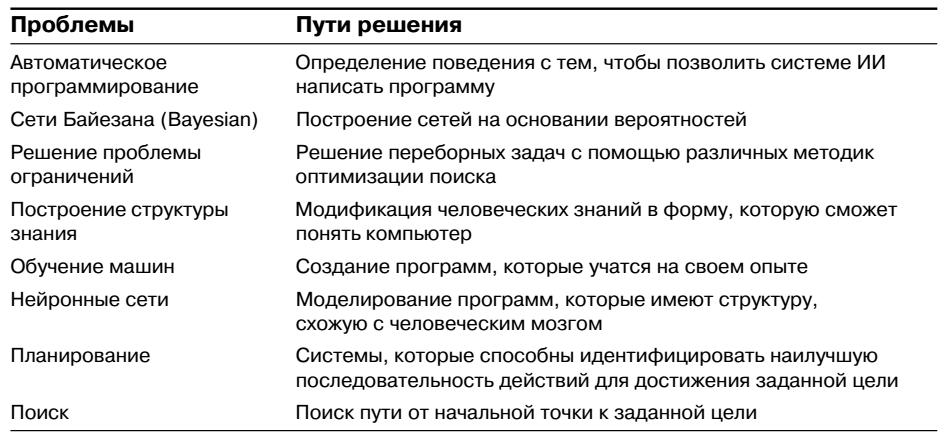
\includegraphics[scale=0.45]{images/lec01-pic02.png}
\end{figure}
\end{frame}

\section{Построение интеллектуальных машин}

\begin{frame}[t]{Построение интеллектуальных машин}
\textbf{Имеющийся ресурс}: большой объем структурированных и неструктурированных данных.

\textbf{Задача}: разработку самообучающихся алгоритмов для приобретения из этих данных знаний с целью выполнения прогнозов.
\begin{itemize}
\item ручной режим: выявлять правила и строить модели на основе анализа
больших объемов данных;
\item машинное обучение (подобласть ИИ):  постепенное улучшение качества прогнозных моделей и принятие решений, управляемых данными.
\end{itemize}
\begin{figure}[h]
\centering
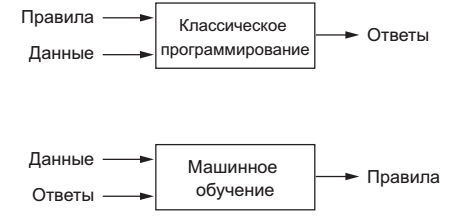
\includegraphics[scale=0.4]{images/lec01-pic12.png}
\end{figure}
\end{frame}

\begin{frame}[t]{Три типа обучения}
\begin{figure}[h]
\centering
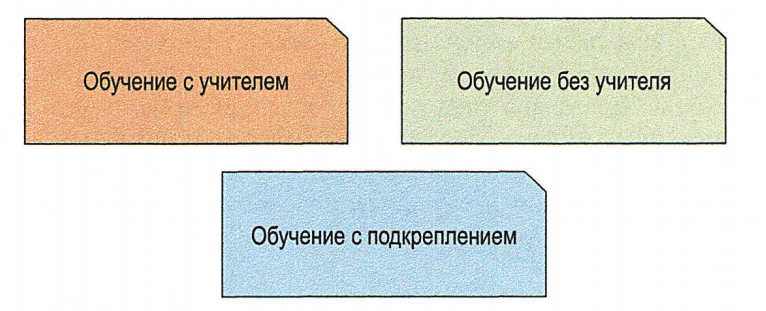
\includegraphics[scale=0.3]{images/lec01-pic03.png}
\end{figure}
\begin{itemize}
\item обучение с учителем: мы знаем правильный ответ заранее; 
\item обучение с подкреплением: мы определяем меру вознаграждения отдельно взятые действия;
\item обучение без учителя: выделение содержательной информации без контроля со стороны известной результирующей переменной или функции вознаграждения.
\end{itemize}
\end{frame}

\begin{frame}[t]{Выполнение прогнозов о будущем на основе обучения с учителем}
\textbf{Задача} обучения с учителем: на маркированных тренировочных данных извлечь модель, которая позволяет делать прогнозы о ранее не встречавшихся или будущих данных.

\textbf{Учитель}: подмножество образцов, в которых нужные выходные сигналы (метки) уже известны.

Пример: фильтрация "спама"
\begin{itemize}
\item методы классификации: имеются дискретные метки принадлежности к классу;
\item регрессия: результирующий сигнал - непрерывная величина.
\end{itemize}
\end{frame}

\begin{frame}[t]{Выполнение прогнозов о будущем на основе обучения с учителем}
\begin{figure}[h]
\centering
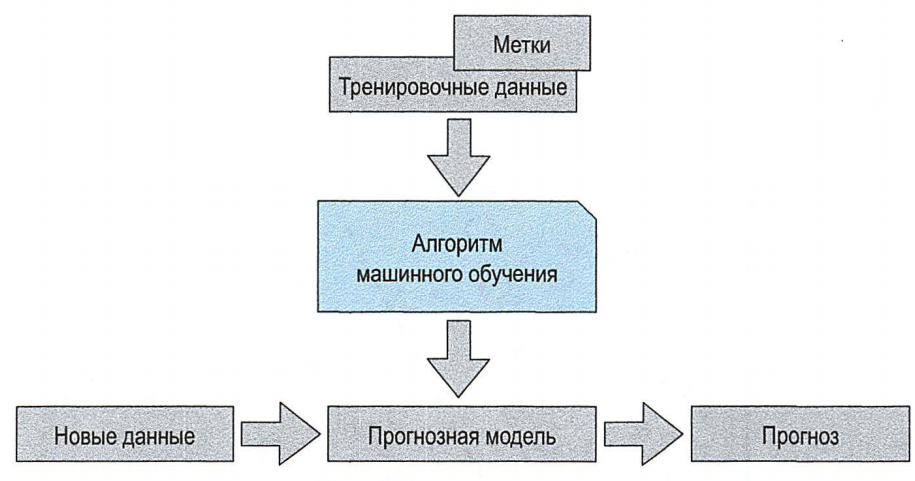
\includegraphics[scale=0.5]{images/lec01-pic04.png}
\end{figure}
\end{frame}

\begin{frame}[t]{Выполнение прогнозов о будущем на основе обучения с учителем}
\begin{block}{Задача классификации}
подкатегория методов машинного обучения с учителем, суть которой заключается в идентификации категориальных меток классов для новых экземпляров на основе предыдущих наблюдений.
\end{block}
Пример: распознование рукописного текста.
\begin{figure}[h]
\centering
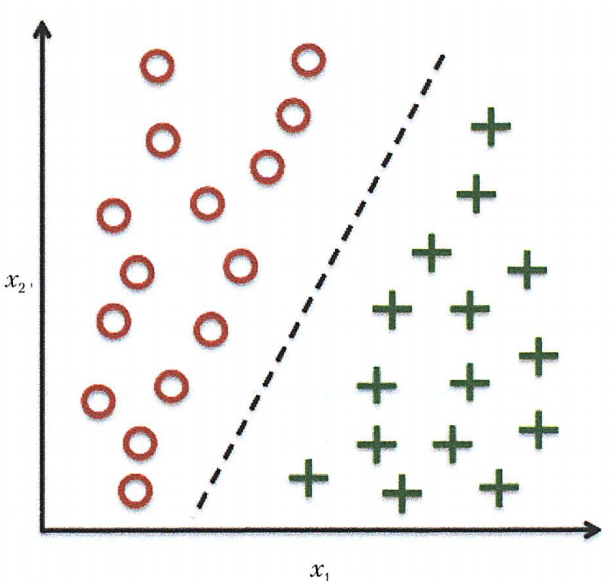
\includegraphics[scale=0.25]{images/lec01-pic05.png}
\end{figure}
\end{frame}

\begin{frame}[t]{Выполнение прогнозов о будущем на основе обучения с учителем}
\begin{block}{Задача регрессии}
предсказанием непрерывных результатов.
\end{block}
В регрессионном анализе нам даны несколько предикторных (объясняющих) переменных и непрерывная (результирующая) переменная отклика, и мы пытаемся найти между этими переменными связь, которая позволит нам предсказывать результат.
\begin{figure}[h]
\centering
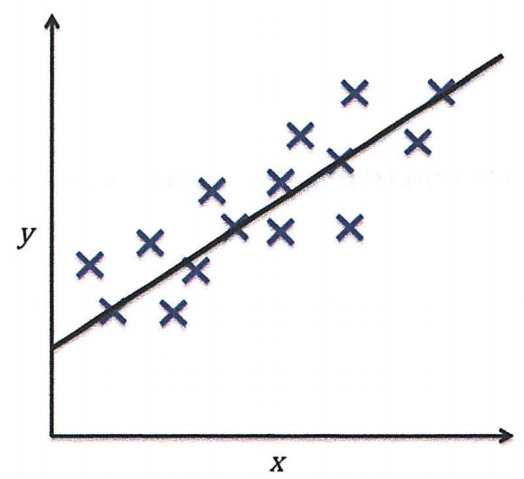
\includegraphics[scale=0.25]{images/lec01-pic06.png}
\end{figure}
\end{frame}

\begin{frame}[t]{Обучение с подкреплением}
\begin{block}{Задача обучения с подкреплением}
выработка системы (агента), которая улучшает свое качество на основе взаимодействий со средой.
\end{block}
\begin{itemize}
\item информация о текущем состоянии среды, как правило, содержит так называемый сигнал вознаграждения, обучение с подкреплением можно представить как область, имеющую отношение к обучению с учителем.
\item обратная связь является не меткой или значением, раз и навсегда определенными в результате прямых наблюдений, а мерой того, насколько хорошо действие было оценено функцией вознаграждения.
\end{itemize}
\end{frame}

\begin{frame}[t]{Обучение с подкреплением}
\begin{figure}[h]
\centering
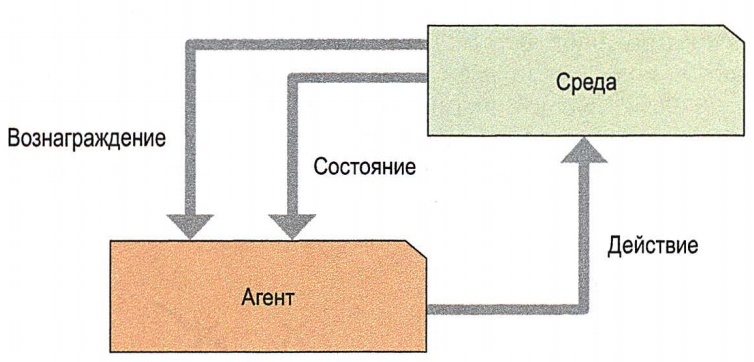
\includegraphics[scale=0.5]{images/lec01-pic07.png}
\end{figure}
\end{frame}

\begin{frame}[t]{Обучение без учителя}
\begin{block}{Кластеризация}
метод разведочного анализа данных, который позволяет организовать груду информации в содержательные подгруппы (кластеры), не имея никаких предварительных сведений о принадлежности группе.
\end{block}
\begin{figure}[h]
\centering
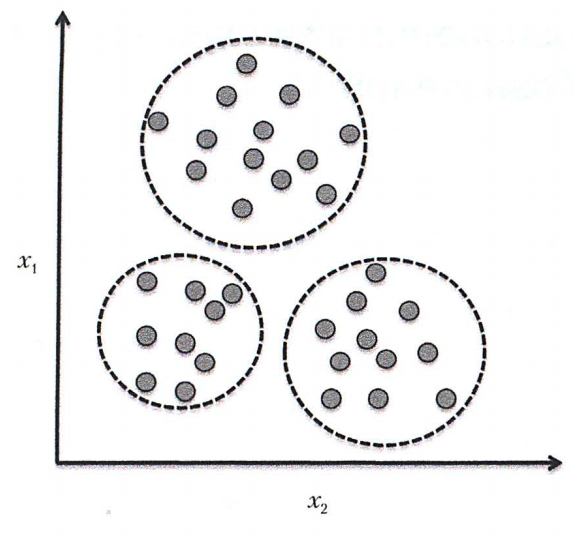
\includegraphics[scale=0.35]{images/lec01-pic08.png}
\end{figure}
\end{frame}

\begin{frame}[t]{Обучение без учителя}
\begin{block}{Снижение размерности данных}
подход, использующийся во время предобработки признаков с целью удаления из данных шума, который тоже может ухудшить предсказательную способность алгоритмов, а также для сжатия данных в подпространство меньшей размерности при сохранении большей части релевантной информации.
\end{block}
\begin{figure}[h]
\centering
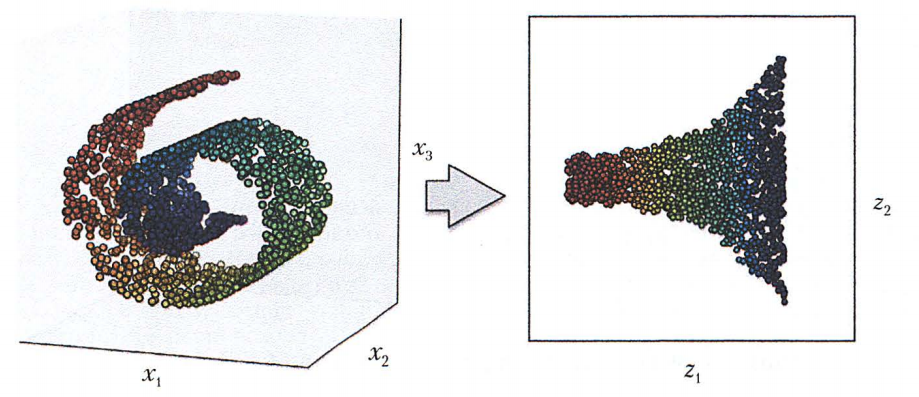
\includegraphics[scale=0.35]{images/lec01-pic09.png}
\end{figure}
\end{frame}

\section{Терминология и система обозначений}
\begin{frame}[t]
Ирисы Фишера (Iris) - набор данных для задачи классификации, на примере которого Рональд Фишер в 1936 году продемонстрировал разработанный им метод дискриминантного анализа. 
\begin{figure}[h]
\centering
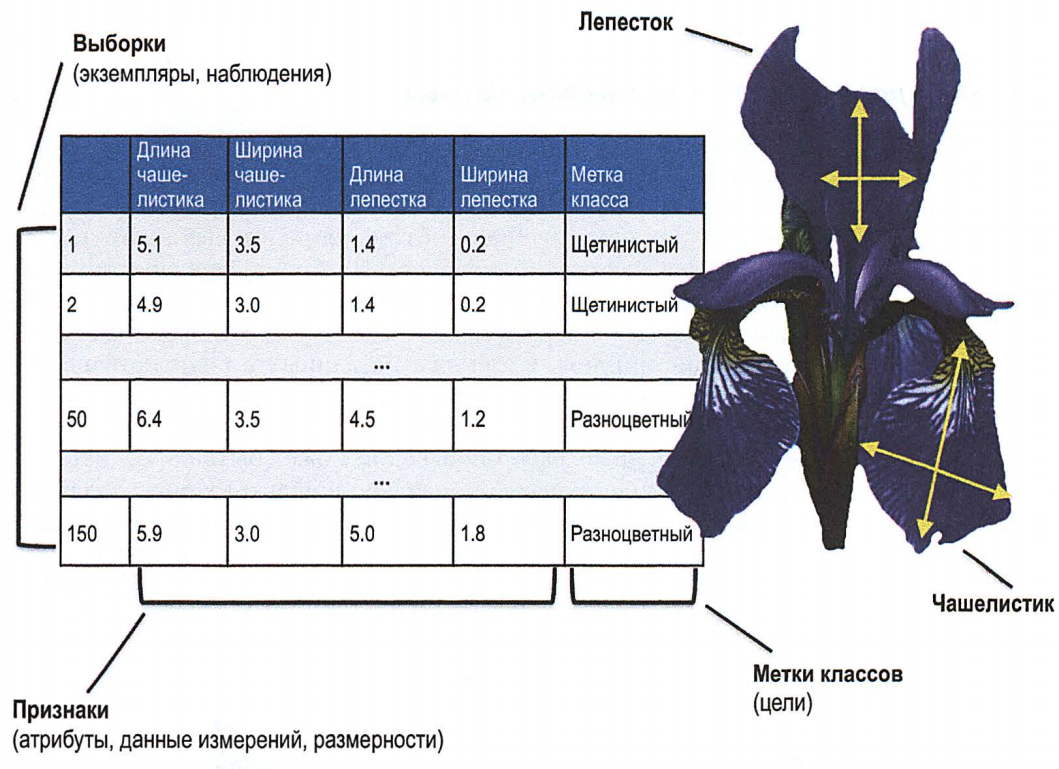
\includegraphics[scale=0.35]{images/lec01-pic10.png}
\end{figure}
\end{frame}

\section{Дорожная карта для построения систем обучения}
\begin{frame}[t]
\begin{figure}[h]
\centering
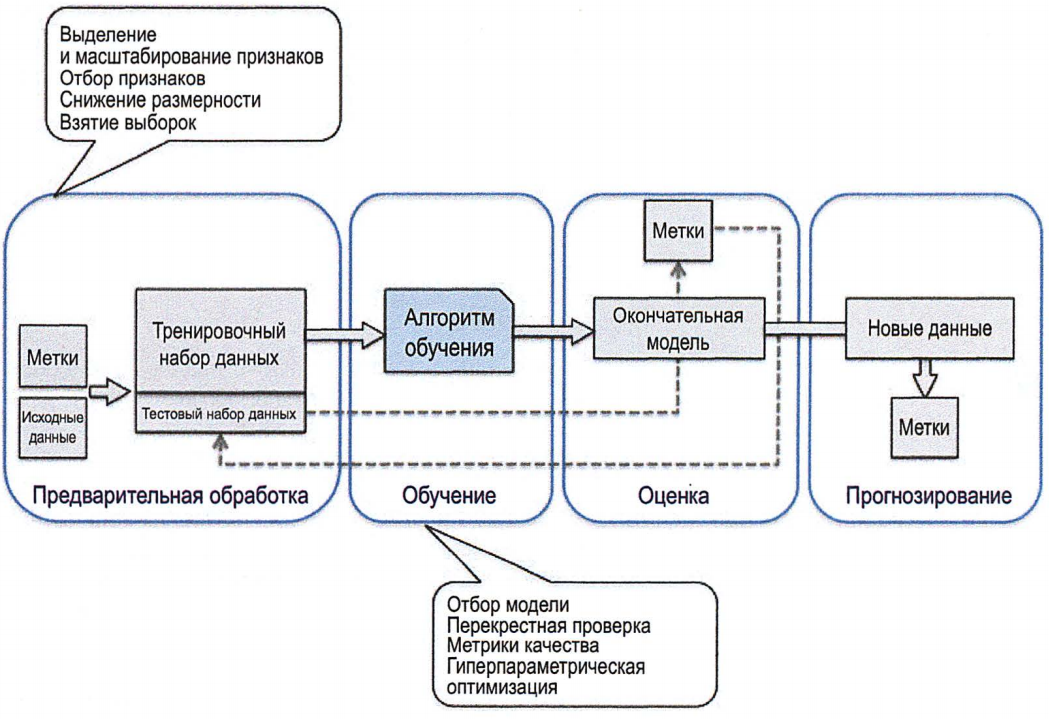
\includegraphics[scale=0.4]{images/lec01-pic11.png}
\end{figure}
\end{frame}

\section{Основные программно-аппаратные реализации}
\begin{frame}[t]{Основные программно-аппаратные реализации}
\begin{figure}[h]
\centering
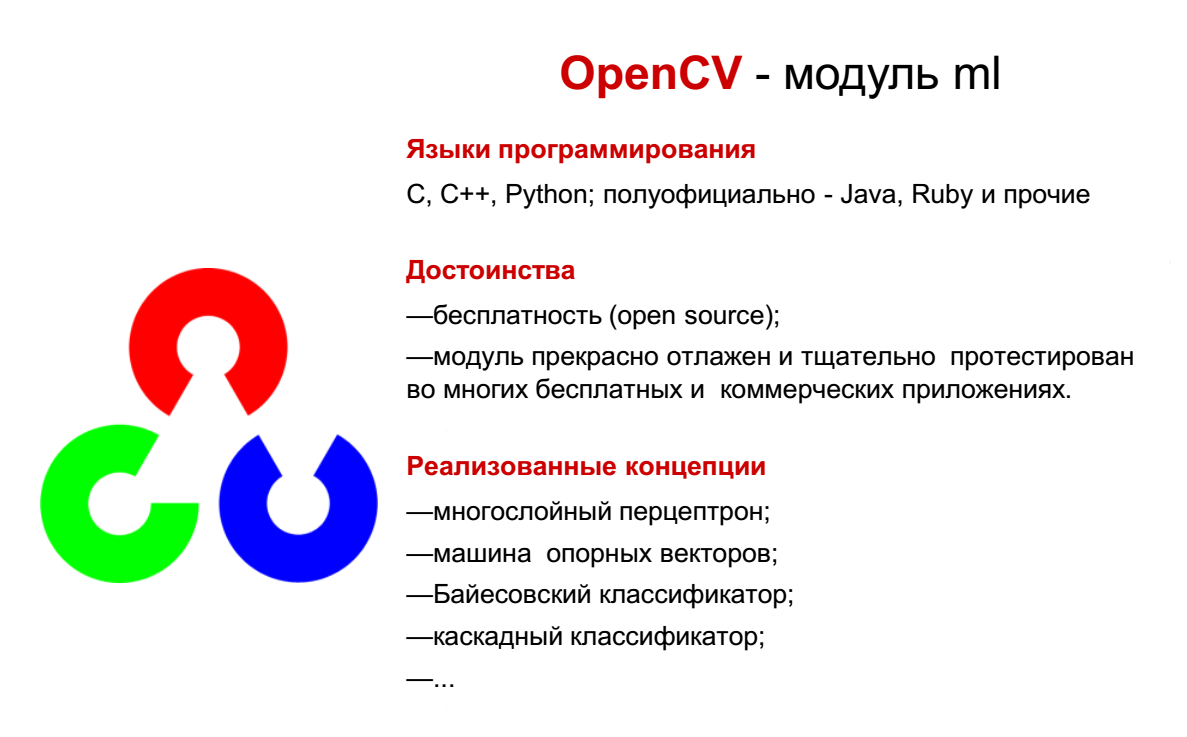
\includegraphics[scale=0.35]{images/lec01-pic13.png}
\end{figure}
\end{frame}

\begin{frame}[t]{Основные программно-аппаратные реализации}
\begin{figure}[h]
\centering
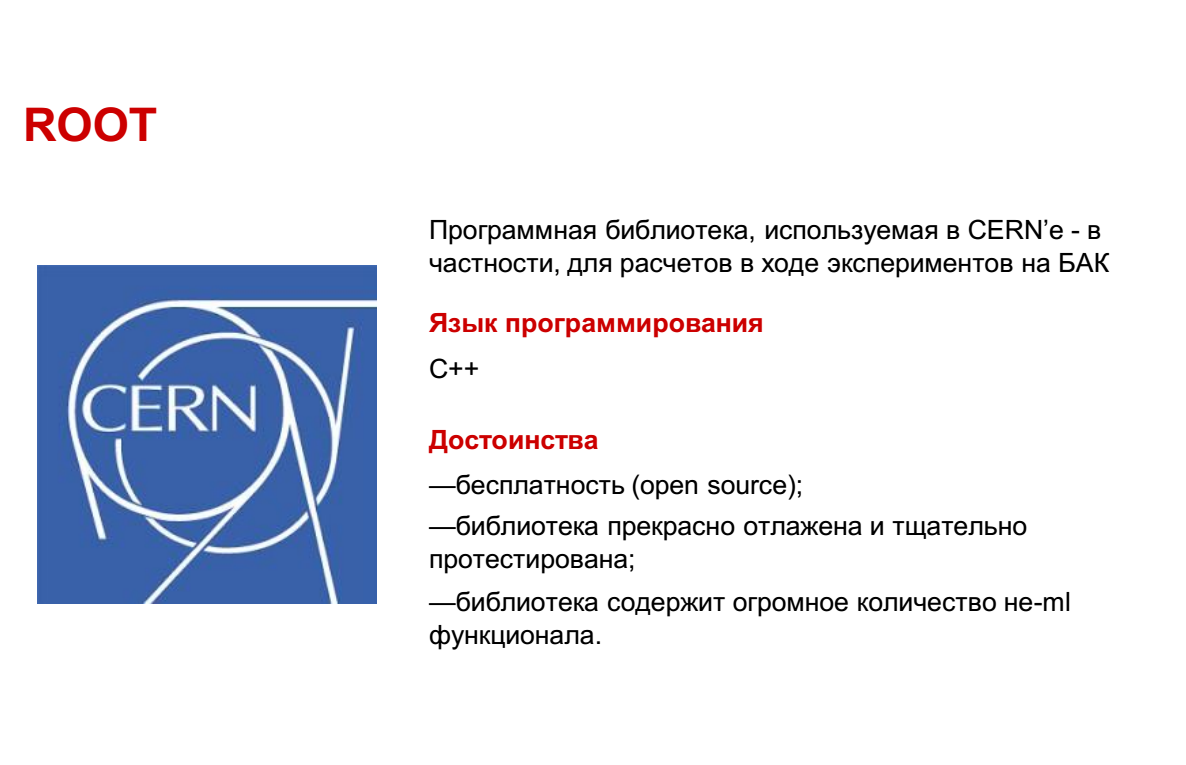
\includegraphics[scale=0.35]{images/lec01-pic14.png}
\end{figure}
\end{frame}

\begin{frame}[t]{Основные программно-аппаратные реализации}
\begin{figure}[h]
\centering
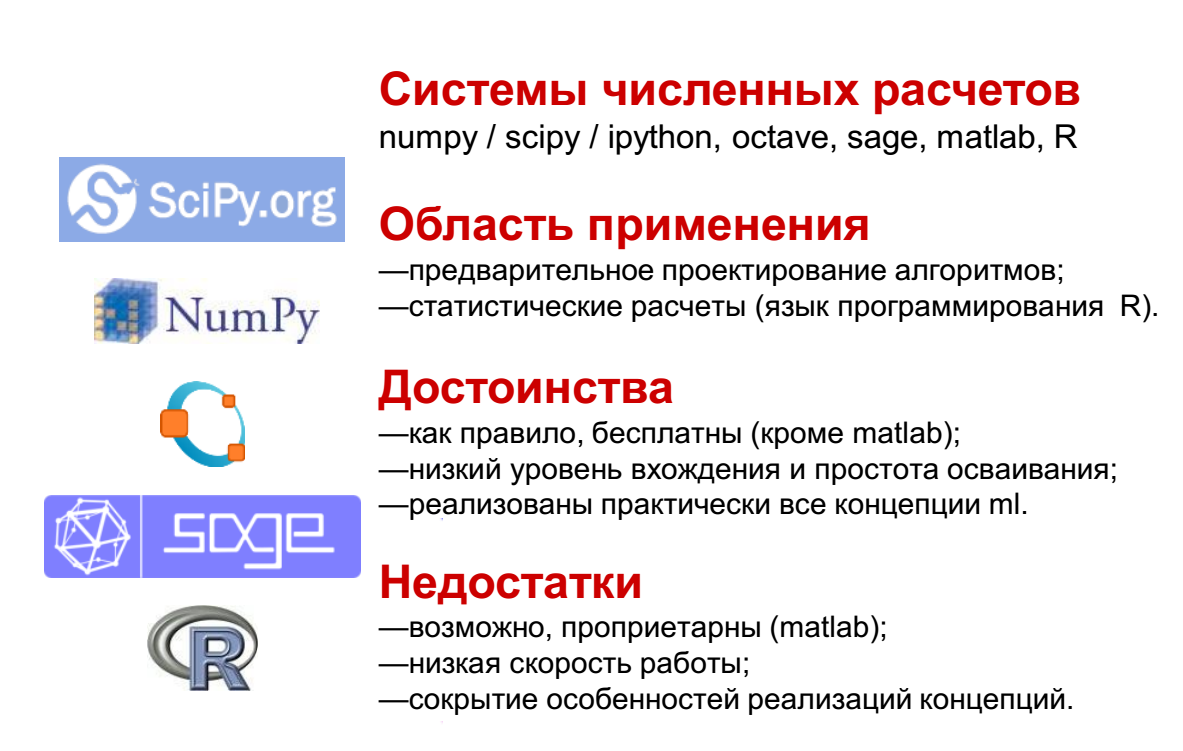
\includegraphics[scale=0.35]{images/lec01-pic15.png}
\end{figure}
\end{frame}

\begin{frame}[t]{Основные программно-аппаратные реализации}
\begin{figure}[h]
\centering
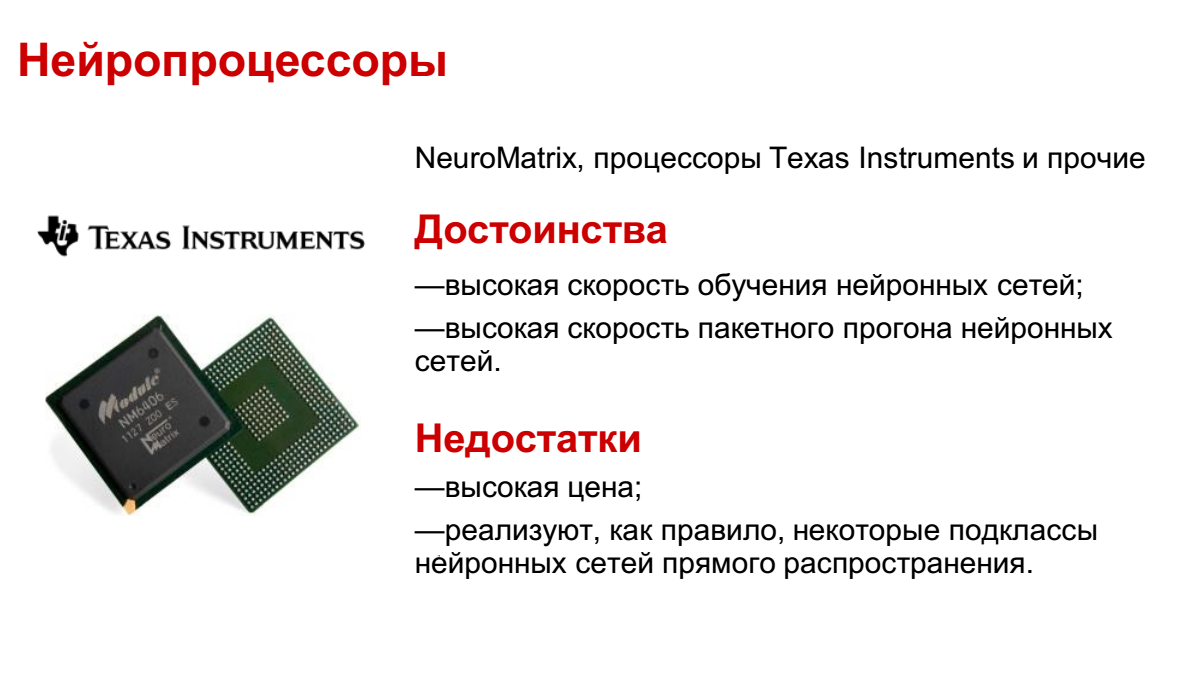
\includegraphics[scale=0.35]{images/lec01-pic16.png}
\end{figure}
\end{frame}

\end{document}
